\documentclass[a4paper, 11pt]{article}

\usepackage{graphicx}
\usepackage{hyperref}
\usepackage[utf8]{inputenc}
\usepackage{minted}

\begin{document}

\title{
	\textbf{Arrays and performance in C}
}
\author{Neo Gullberg}
\date{Fall 2024}
\maketitle

\section{Introduction}
	In this assignment my task was to benchmark three different operations on arrays in the C programming language.
	After creating and executing the benchmarks, and measuring their performance, I had to present and explain the results.
	I also had to find polynomials in big O notation that roughly described the time complexity for a given operation for an array of size \textit{n}.

\section{To Measure Time in C}
	Before any benchmarking of performance can take place there has to be a way to measure time.
	A code snippet for how to do this was given to us in the instructions, with the included task of figuring out the clocks accuracy.
	From my naive approach, of just running the program a bunch of times, I measured the minimum time taken, between starting and stopping the clock, to be around 10 ns.
	The reason why we are only interested in finding the minimum amount of time it can take is because there is a definite least amount of time it HAS to take, whilst the maximum
	amount of time it \textit{could} take has no limit. The maximum can grow to be very large since the operating system sometimes has to prioritize other running processes
	between us starting and stopping the clock which affects our measurements.
	However, the minimum time could \textit{never} be zero (or negative) since the physical clock of a computer ticks at a fixed rate which conforms to the laws of physics.
	\par
	If we want to try and measure the time it takes for a single array access,
	we immediatly run into the problem that the time it takes to \textit{measure time} far outweighs the time it takes to actually access an element of an array.
	We mitigate this by performing a large amount of array accesses and measuring them all together.
	If done in large enough quantities this solves our problem.
	I found that performing around 100 array accesses was enough to mitigate the uncerainty of the clock.

\section{Random Access}
	Why we want to specifically benchmark random accesses from an array instead of sequential accesses is because
	we want to minimize the performance benefit that the CPU cache would otherwise bring.
	\par
	\begin{figure}[h]
		\centering
		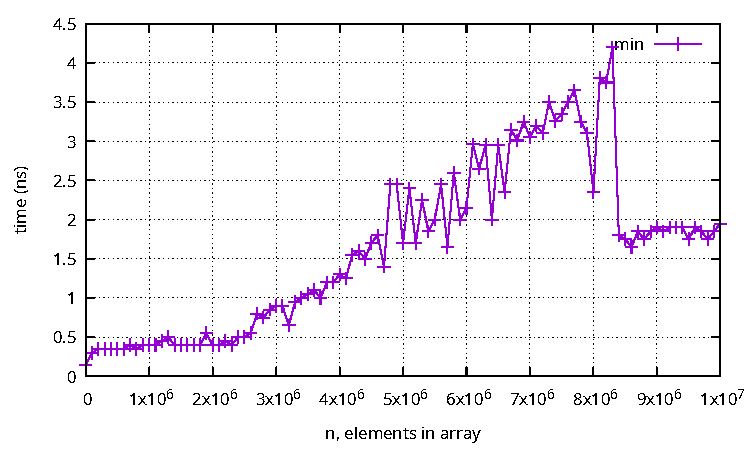
\includegraphics[scale=0.8]{graphs/plot2_10,000,000.pdf}
		\caption{
			Graph showing the time it took to access a random element in an array of size \textit{n}, up to \(n=10,000,000\).
		}
	\end{figure}
	This first graph seems to be all over the place. However, if we look at the start of the graph we see the measurements there to be fairly stable.
	Therefore, I made another graph with a smaller range.
	\par
	\begin{figure}[h]
		\centering
		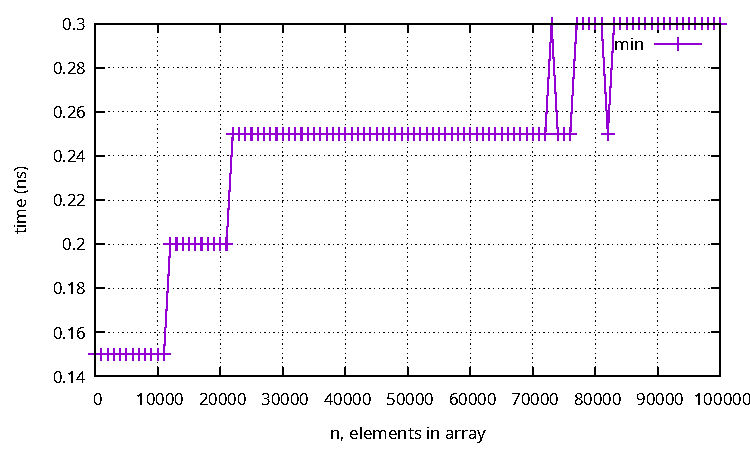
\includegraphics[scale=0.8]{graphs/plot2_100,000.pdf}
		\caption{
			Graph showing the time it took to access a random element in an array of size \textit{n}, up to \(n=100,000\).
		}
	\end{figure}
	In the second graph we get a clearer look at how the access times look like in the beginning.
	An interesting pattern seems to arise where stable plateaus are separated by spikes.
	The bigger the size of the array, the more unstable the measurments become.
	The first spikes I belive to be caused by cache misses closest to the CPU, in its L1-L3 caches maybe.
	The further out we get the more prevalent the cache misses become.
	After around the \(100,000\) mark it looks like the CPU maybe has to start fetching from RAM, which is much more expensive compared to the cache.
	\par
	In the early stages the randomness is not as noticable since the CPU has a very high change (if not 100\%) to have the whole array stored directly in the cache.
	This means, for arrays that fit entirely in the cache the time complexity of accessing a random element is roughly \(O(1)\).
	Once the array grows large enough (which differs between hardware) the random access times start to increase and fluctuate more.

\section{Search for an Item}
	The supplied algorithm for searching for an item was very simple.
	It generated a random value and then compared it to all elements of an unsorted array of size \textit{n}
	until it found a match or reached the end.
	The range of these random values were \([0, 2n - 1]\) so that there would exist a possibilty for there to be no match.
	If the range would have been smaller than the size of the array, there would always have been a guaranteed match somewhere in the array.
	\par
	\begin{figure}[h]
		\centering
		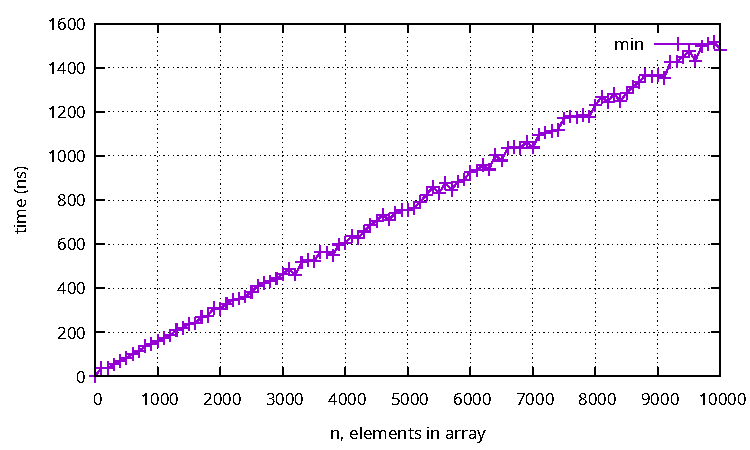
\includegraphics[scale=0.8]{graphs/plot3.pdf}
		\caption{
			Graph showing the time it took to search for a specific item in an array of size \textit{n}.
		}
	\end{figure}
	The graph shows us that the time complexity of searching for an item in an array with the supplied algorithm is roughly \(O(n)\).
	This makes sense as the algorithm does not make use of any clever tricks to improve the search, it merely brute-forces its way through the array.
	Over the span of multiple iterations the random search time should average out and find an equilibrium time relative to \textit{n},
	which is what we can see hold true throughout the graph. This is why it's very important to perform multiple iterations,
	since otherwise our graph would look like a jumbled mess because the search times would not even out and therefore be completely random.
	That would mean we would not be able to draw a clear conclusion from our measurements.

\section{Search for Duplicates}
	The supplied algorithm for searching for duplicate items between two arrays, of the same size, makes us of the same brute-force search algorithm as the last operation.
	For every item in the first array it searches through the second array until it either finds a match or reaches the end.
	\par
	\begin{figure}[h]
		\centering
		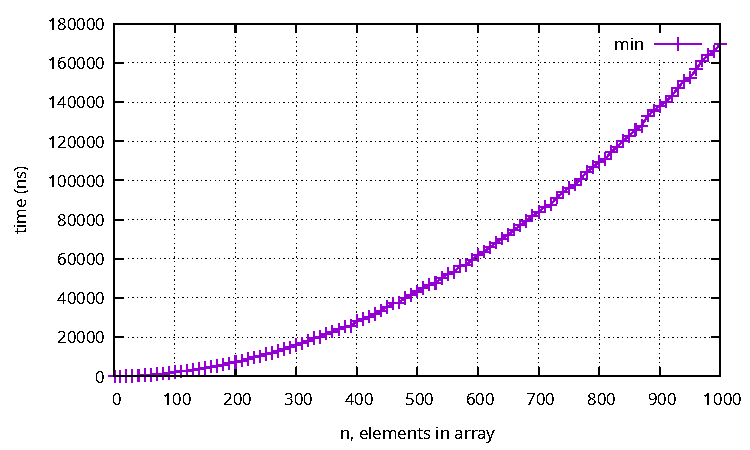
\includegraphics[scale=0.8]{graphs/plot4.pdf}
		\caption{
			Graph showing the time it took to search for duplicates between two arrays of size \textit{n}.
		}
	\end{figure}
	The graph shows us that the time complexity of searching for duplicate items between two arrays, of the same size, is roughly \(O(n^2)\).
	This operation is using the previous search operation, which we saw had a time complexity \(O(n)\), and performing it \textit{n} times.
	Basic multiplication tells us that \(n \times n = n^2\), which gives us a final time complexity of \(O(n^2)\).

\section{Source Code}
	If anyone is interested, the code I used to benchmark these operations and generate the graphs can be found over at: \url{https://github.com/neogulgul/ID1021/tree/main/Intro/program}

\end{document}
